For a better insight into the project, it is necessary to introduce certain theoretical concepts first. In the next chapter this theory will be used to base the approach on for the design and development of the algorithm and choices regarding the proof of concept.

\subsection{Drive-by downloads}

Browsing the internet with an unpatched system, for example because the patch is not installed or there is simply no solution available, can be dangerous. All software contains mistakes and such mistakes are patched almost on a daily basis. Part of those mistakes can be (ab)used to get control over a computer system and be used to run malicious software without the user noticing.

If a website uses such mistake to take control over the web browser and download malicious software to the system, this is called a drive-by download\cite{Le2013}. Figure \ref{fig:dbdownload} shows the steps involved from visiting a website until the moment the system is infected with malware.

By compromising the web browser and injecting malicious code, the malware gets full control over the infected process, running with the same privileges as the web browser on the host system. Depending on the system configuration this either means that full system access is available or that additional steps are required to escalate the privileges to the intended level.


\begin{figure}[h]
    \centering
    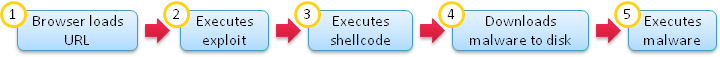
\includegraphics[width=12cm]{Images/drive-by-download.png}
    \caption{The anatomy of a drive-by download malware infection. \cite{dbdownload-anatomy}}
    \label{fig:dbdownload}
\end{figure}

\subsubsection{behaviour}

What happens after a malware infection depends on the malware used and goals of the attacker. In many cases the malware will download further malicious components and nestle itself in the operating system so it can be restarted after a reboot of the operating system and is able to restore itself after an attempt to remove it.

To do this, the malware modifies, for example, files and registry values or performs network operations. While theoretically malware could directly communicate with the kernel for this, most malware\todo{need citation} behaves like a normal application and uses the installed, or with the operating system provided, libraries. The usage of such libraries can be detected when the access to them is monitored.

\subsection{API analysis}

In the early days, libraries were primarily used by an application by statically linking to it. This means that the library becomes part of the application and it is no longer possible to determine which part of the application was originally part of the used libraries.

For performance and maintainability, dynamic linking was invented. The application describes which libraries it needs and the linker of the operating system will glue the applications and its dependent libraries together in the memory space of the application. 

Because the linker has to know all exported functions and where in the library it can find such function, a symbol table is part of every dynamic library. The same information can be used to hook into an provided function during runtime or to trick the linker to load a replacement of a certain function because the modified version has a higher priority.

This is called API hooking\cite{} and it is a very useful technique to monitor the behaviour of applications. The original function is replaced by a substitute. This substitute function calls, for example, the original function and logs the performed operation or \todo{change sentence} is a custom replacement of the original function.

The technical implementation of API hooking is highly complex and platform specific. Many different techniques\cite{jbremer2012} of hooking are possible as well. If the start of the application can be controlled, the linker search path can be extended to include the replacement library. Alternatively, the import section of the application can be modified. When the application is already loaded or modification of the application or system is unwanted, the function to hook can be overwritten in memory with a replacement or jump to a different location in memory. However, this will prevent the ability to execute the original function unless the overwritten bytes are carefully preserved and reconstructed somewhere else.

In this project API hooking will be used to reverse engineer the internal workings and API usage of web browsers and to log the behaviour of malware for later analysis.

\subsection{Web browser architecture}
% Target: 4-6 blz

\todo{Meer bronnen?}

Modern web browsers are complex applications consisting of many components which have to work together. To develop a generic algorithm, it is crucial to have an in-depth understanding of the inner workings of a web browser. This project focuses on Internet Explorer, Mozilla Firefox, Chromium and Apple Safari. Those four browsers combined have a marketshare of more than 90\%\footnote{http://gs.statcounter.com/\#desktop-browser-ww-monthly-201412-201412-bar} \footnote{http://www.netmarketshare.com/browser-market-share.aspx?qprid=1\&qpcustomb=0}.

All modern web browsers allow the usage of multiple tabs in a single window. The underlying implementations of those tabs differ greatly. Internet Explorer and Safari use only libraries provided by the operating system while Firefox and Chromium decided to use their own libraries. Some browsers decided to use multiple processes and sometimes even a new process for every single tab.

\textbf{Internet Explorer} supports tabs since version 7 and version 8 was improved with the ability to run tabs in their own process (see figure \ref{fig:ie8proc}). This feature is called ``loosely-coupled IE''\cite{IE8LCIE}. Every process runs independent from the other processes and runs with its own network stack and instances of content plugins like Flash or Silverlight.

Starting each tab in its own process comes with an inevitable overhead of using more memory and a slower startup. For this reason a process in Internet Explorer can host multiple tabs. The amount of tabs in a single process and the maximum number of processes is determined by the configuration. For backwards compatibility, Internet Explorer also provides the option to disable the usage of multiple processes and host all tabs in a single browser process.

\label{sec:brie}
The network stack used in Internet Explorer is provided by the Windows operating system and is called WinINet\cite{wininet}. This library provides high-level access to functions that allow HTTP and FTP requests and utility functions for caching, proxies and security. After initiating and configuring the request, WinINet will perform the necessary steps to execute the request. WinINet depends on the Winsock library \cite{winsock} to setup the required network connections and Schannel \cite{schannel} is used to provide transparent support for SSL/TLS connections.

\begin{figure}
    \centering
    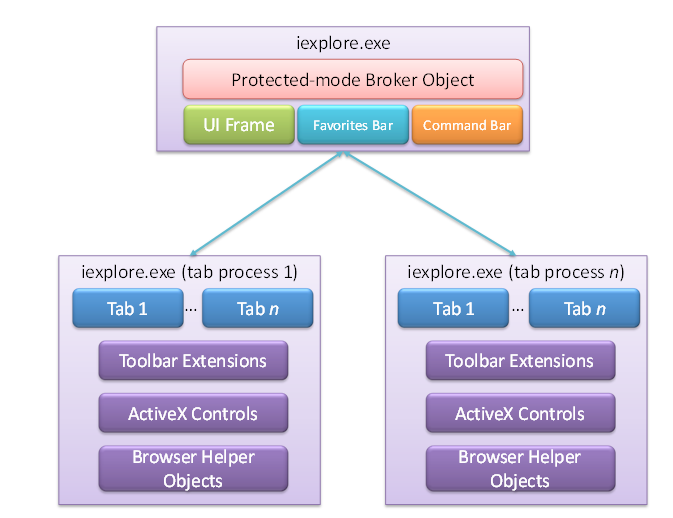
\includegraphics[width=9cm]{Images/IE8_process_model.png}
    \caption{The Internet Explorer process model starting from version 8. \cite{IE8LCIEP}}
    \label{fig:ie8proc}
\end{figure}

\textbf{Firefox} uses only a single process for web content and only runs plugins from a different process. A long-term project to change that is called Electrolysis\footnote{https://wiki.mozilla.org/Electrolysis} and has been developed since 2009. In the new architecture, the entire rendering moved to a dedicated and sandboxed ``content'' process and the main process is used to host the user interface and serves as a proxy between the outside world and the content process. A longer-term goal is to spread the rendering of multiple tabs over more than one content process so when a content process crashes not all tabs are affected.

To be platform independent, Firefox does not directly interface with the provided libraries of the operating system. Instead a platform-neutral API called ``NSPR'' (Netscape Portable Runtime, \cite{nspr}) is used. Together with the Network Security Services (NSS, \cite{nss}) library that provides the functionality to create SSL/TLS connections, both are used by the high-level network library called Necko. Necko provides the interface to perform HTTP and other protocol requests without revealing the underlying protocol, transport level or platform specific implementation details and is thus comparable to WinINet.

\textbf{Chromium} is the open-source version of the Google Chrome browser and it is except for a couple of proprietary components identical to Chrome. The big innovation of Chrome \cite{ChromeMPA} was to use multiple processes instead of a single process. Besides its own process for every tab, it also has the plugins and audio subsystem in their respective processes. The subprocesses run in a sandbox with limited privileges and use the main process to communicate with the outside world.

\begin{figure}[h]
    \centering
    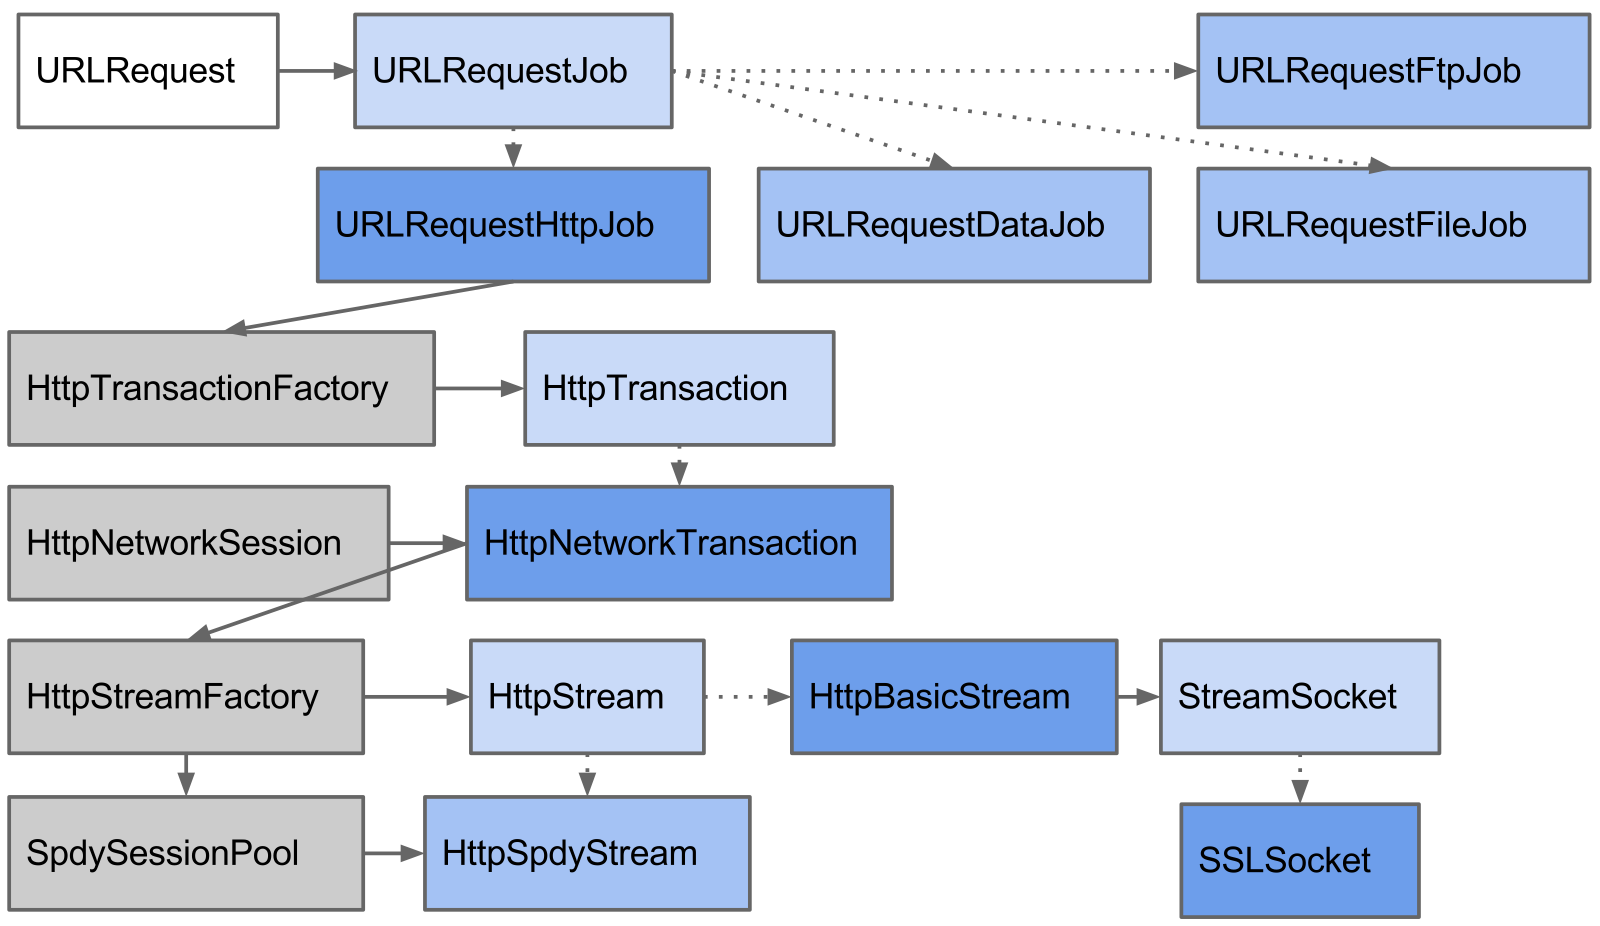
\includegraphics[width=9cm]{Images/Chrome_network.png}
    \caption{A high-level overview of the components involved in requesting an URL in Chromium. Platform specific details related to sockets are hidden in StreamSocket and the usage of SSL/TLS is made transparent by using the interface-compatible SSLSocket instead of StreamSocket. \cite{ChromeNetwork}}
    \label{fig:chrome_network}
\end{figure}

The library used by Chromium for network access is custom developed and tightly integrated in the engine. It provides similarly functionality as Necko and WinINet using a high-level interface (see figure \ref{fig:chrome_network}) but also it contains low-level interfaces that interface directly with the operating system's socket API. To provide transparent SSL/TLS support, the same library as Firefox is used, NSS.

\textbf{Safari} is the last browser that was examined in this project. Since 2011\footnote{https://lists.webkit.org/pipermail/webkit-help/2011-July/002298.html} support for using multiple processes has been added. Safari is closed-source but build on top of many open-source components like JavaScriptCore and WebKit.

Safari uses a dedicated process for every tab until a certain limit is reached. Once this limit is reached, multiple tabs are hosted in a single process. The network operations for the main and tab processes is concentrated in a dedicated process. Only this process will retrieve the webpages and use IPC mechanics to deliver the result to the correct process. 

CFNetwork is the library that is used by Safari for its network access. This library is one of the core frameworks of the OS X operating system and available for all applications. It provides interfaces for all relevant web related protocols. A unified interface called NSUrl, similarily to other browsers, is also available. However, because of the closed-source nature of Safari it is not possible without an extensive reverse engineering effort to determine if it is used instead of directly using the provided APIs of the CFNetwork library.

\iffalse

Which techniques are used by browsers to make concurrently visiting multiple
URLs possible?
	- Tabs of course
		- As a process
		- As multiple threads under the browser process

How can we link an HTTP request to its source URL without the modification of the used web browser?
we need extra information, see vraag 4
network is niet genoeg blablabla

How do web browsers make HTTP requests and retrieve webpages? Which Operating System level APIs are used?
	- Safari: CFNetwork and NSURLConnection(Loader) and IPC
		1 hoofdprocess: Safari
		1 process per tab: Safari Web Content
		1 process voor networking: Safari Networking
		Network stack of OS X.
	- Internet Explorer: C API calls naar Windows libraries
		Process per tab: is configureerbaar in settings/registry, je kan ook meerdere tabs in 1 process hebben
		Network stack of Windows
	- Firefox: C++ Library calls
		Single Process (+ 1 process voor flash)
		Own network stack Necko (nss3 voor trafiek te encrypten)
		\url{https://developer.mozilla.org/en-US/Firefox/Releases/3.5/Updating_extensions#Getting_a_load_context_from_a_request}
		http://stackoverflow.com/questions/10719606/is-it-possible-to-know-the-target-domwindow-for-an-httprequest
	- Chrome: IPC 
		1 hoofdprocess: Google Chrome die networking doet
		1 process per tab. (Altijd 13 threads?)
		1 process voor Flash.
		1 process voor Audio. (4 threads)
		Own network stack (nss3 voor trafiek te encrypten)
		http://www.chromium.org/developers/design-documents/network-stack

What extra information from the client's (running) machine can be used to augment the information gained from network trac to make the tracking of malware to its source URL easier?  
	- The Thread ID or Process ID van tabs, PDF reader, Java applet, ...
	- Handle bij IE
	- File descriptors
	- Process tree
	- Voordeel van op machine network traffic te intercepten is dat we rommel van andere applicaties niet zien, maar enkel het trafiek van de browser en de gespawnde subprocessen ervan.
	- 
\fi

